\documentclass[conference]{IEEEtran}
\IEEEoverridecommandlockouts
% The preceding line is only needed to identify funding in the first footnote. If that is unneeded, please comment it out.
\usepackage{cite}
\usepackage{amsmath,amssymb,amsfonts}
\usepackage{algorithmic}
\usepackage{graphicx}
\usepackage{textcomp}
\usepackage{xcolor}
\def\BibTeX{{\rm B\kern-.05em{\sc i\kern-.025em b}\kern-.08em
    T\kern-.1667em\lower.7ex\hbox{E}\kern-.125emX}}
\begin{document}

\title{Mastering 2048 game\\
}

\author{\IEEEauthorblockN{Daniele Foschi}
\IEEEauthorblockA{\textit{Alma Mater Studiorum Università di Bologna} \\
\textit{UNIBO}\\
Bologna, Italy \\
daniele.foschi2@studio.unibo.it\\
https://github.com/DaniDF/RL\_reinforce\_2048\_aas}
}

\maketitle

\begin{abstract}
2048 is a highly addictive sliding puzzle video game developed by Gabriele Cirulli in 2014. The game quickly gained popularity, and players began to challenge each other to achieve the highest score. This dissertation discusses different AI-based agents for playing the game and achieving the goal of reaching the 2048 tile.
\end{abstract}

\begin{IEEEkeywords}
2048, game, reinfoce
\end{IEEEkeywords}

\section{Introduction}
The release of the 2048 game in 2014 sparked a surge in popularity among players and research interest in building the best AI-based agent for the game.
The AI-based agents discussed in the dissertation are policy gradient agents with baselines. These agents select an action at each step by maximizing the expected return. The baseline is an estimate of the expected return for a given state, and it is used to reduce variance in the policy gradient updates. The dissertation explores different approaches to training policy gradient agents, with the goal of training the best possible agent for playing 2048.
In the subsequent sections, we will introduce the rules of the 2048 game. We will then present other AI-based solutions that have been proposed for the game. Next, we will describe the architecture of the proposed networks. Finally, we will present the collected results from the training of the networks.


\section{Background}
2048\cite{2048} is a single-player, deterministic, turn-based, sliding puzzle video game developed by Gabriele Cirulli and released in 2014. The game was originally written in JavaScript and later ported to Android and iOS.
The game 2048 is played on a 4x4 grid of cells. At the beginning of the game, the grid is initialized with two non-empty cells. At the beginning of the game, two tiles are randomly placed on the grid with values between 2 and 4. At each step, the player can choose one of four moves: \textit{LEFT}, \textit{UP}, \textit{RIGHT}, or \textit{DOWN}. After a move is played, all tiles are translated in the direction of the action without any intervening spaces between tiles. If two tiles with the same value are adjacent after the translation, they are merged into a single tile with the sum of their values. The game score is then incremented by the value of the new tile.
After the player has completed their move, the game randomly adds a new tile to the board. The game then continues. The game stops when there are no tiles that can be merged and no empty spaces on the board.
The goal of the game is to reach the tile with a value of 2048 on the board. After reaching the 2048 tile, the game does not terminate and allows players to continue to merge tiles and increase the value of the tiles. The maximum tile value is $131072$, which is equal to $2^{17}$. The number of legal board configurations is $18^{16}$.


\section{Related works}
From the release of the game in 2014 a lot of researchers tried to win the game and achieve the 2048 tile on the board.
P. Rodgers and J. Levine\cite{ai-strat} 2014 compared different approach to learning how to win 2048 game and the best strategies. They used Montecarlo Tree Search (MCTS) to estimate the goodness of each bord configuration. They expected at the end of the simulation to have an asymmetric tree, that will result in an easiest situation for concentrating the efforts on the potentially good moves. Instead, they discovered that playing 2048 ends in symmetric trees.
They also implemented Averaged Depth-Limited Search (ADLS), which is an approximation of Expectimax that runs multiple simulations. This approach does not try to simulate all possibilities, but the more likely situations will appear more often in the simulations. They concluded that ADLS is a lot better than MCTS because ADLS uses an evaluating function that is fundamental in a game such as 2048, which has a lot of randomness and where minimizing risks is key.
Marcin Szubert and Wojciech Laskowski\cite{td-after} developed a TD(0)\cite{td} agent, TD-afterstate, that is capable of winning the 2048 game without incorporating human expertise. They showed that TD-afterstate can achieve a win rate of 98\% with a powerful evaluation function. They also highlighted that learning afterstates is a viable way to learn state values in a stochastic environment where it is difficult to obtain the following state.

\section{Implementation}
In order to achieve the goal of getting the 2048 tile on the board this dissertation propose an agent based on the reinforce algorithm. In particular the reinforce algorithm \cite{reinforce} was implemented using neural networks implemented in TensorFlow. In addition a baseline was implemented using another neural network.
Based on the game board, both neural networks are filled in input with a sequentialized version of the board matrix: each row follows the previous one.
Like the neural network’s weights, also the input values are represented using the tf.float32 data type of TensorFlow library.
The first implementation \label{lab:first_net} of the \textit{policy network} is composed by seven hidden layers fully connected with the following nodes $[512,512,256,256,128, 64,64]$. The network used to predict the value (\textit{value network}) has four hidden layers fully connected $[512,512,256,128]$.
This implementation was trained for 200000 episodes.
A second \label{lab:second_net} pair of networks were tested: \textit{policy network} with eight hidden layers fully connected $[2048,2048,1024, 1024, 1024, 1024, 1024, 1024]$ and the \textit{value network} composed by six hidden layers fully connected $[2048,2048,1024, 1024, 1024, 1024]$.
This implementation was trained for 400000 episodes.
After the training both implementations are used to play 10000 games\label{lab:replay} and the ending board configurations, with the five less valuable tiles setted to zero, are used as a starting point for fine-tuning the networks. The played ending states were mixed with new games with probability of 33\%.


\section{Experimental results}
For each network configurations during the training the rewards for each episode are recorded. Every 20000 episodes the top $95^{th}$ percentile is computed.
After each training $1000$ games are played and the highest tile is recorded in other to record if the goal of reaching the 2048 tile is achieved.

\subsection{First implementation}
In the first implementation (see \ref{lab:first_net}) the \textit{policy network} is composed by seven hidden layers fully connected and the \textit{value network} composed by four layers fully connected.
\subsubsection{First training}
$200000$ episodes:
\begin{figure}[htbp]
\centerline{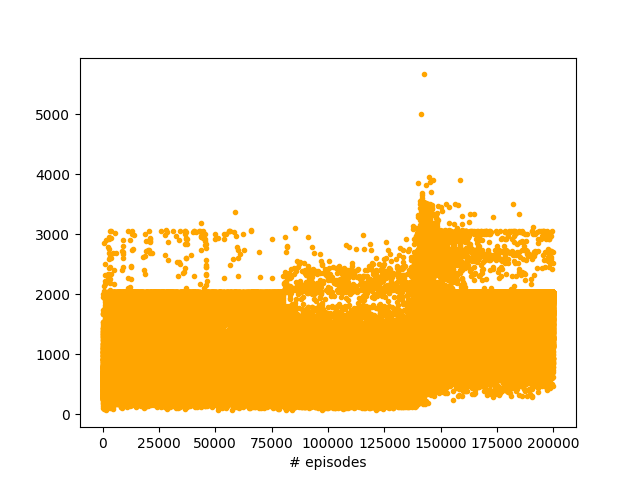
\includegraphics[scale=0.4]{05_experimental_results/05_images/ckpt-#0-1_big-net_rewards.png}}
\caption{Game score}
\label{fig:0-1_reward}
\end{figure}

\begin{figure}[htbp]
\centerline{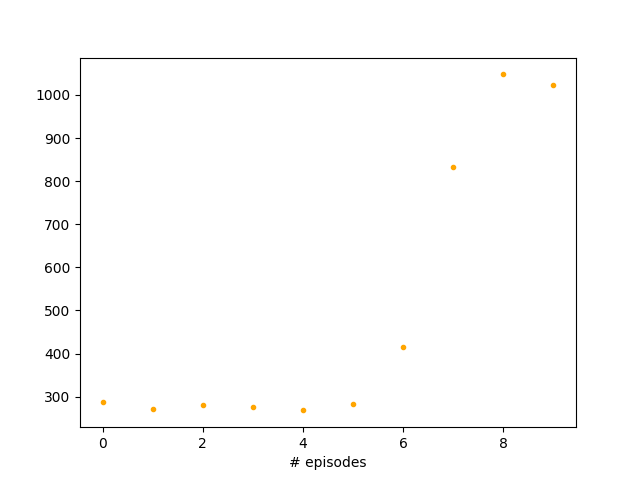
\includegraphics[scale=0.4]{05_experimental_results/05_images/ckpt-#0-1_big-net_compute_percentiles_1000_rewards.png}}
\caption{Top 95 percentile game score, computed every 20000 episodes}
\label{fig:0-1_percentile}
\end{figure}

\begin{figure}[htbp]
\centerline{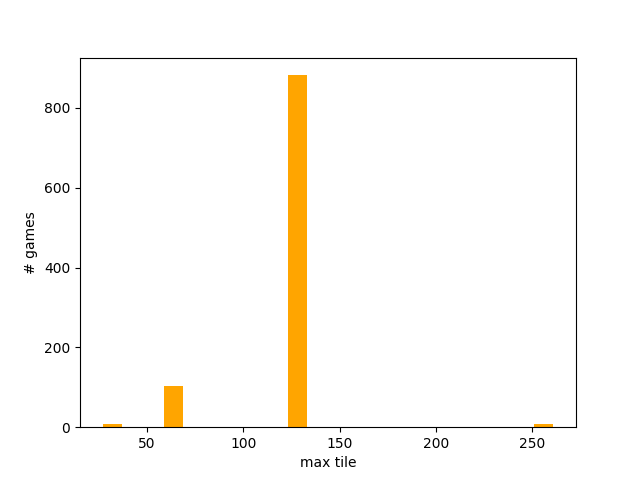
\includegraphics[scale=0.4]{05_experimental_results/05_images/ckpt-#0-1_big-net_play_games_1000_ending_states.png}}
\caption{Number of game with specific max tile's value}
\label{fig:0-1_end_state}
\end{figure}

\\
After this training, the network has learned to exhibit strategic behaviour, such as placing the highest tile in a corner and the following tiles in a diagonal pattern.
The max tile registered is in very few examples 256, still far from the goal of 2048 (fig \ref{fig:0-1_end_state}).
After $120000$ episodes, the distribution of game scores becomes more positively skewed, with a greater proportion of scores occurring at higher values (fig \ref{fig:0-1_percentile}).

\subsubsection{Second training}
$160000$ episodes using as starting board configuration $10000$ played games with probability $33\%$ (see \ref{lab:replay}):
\begin{figure}[htbp]
\centerline{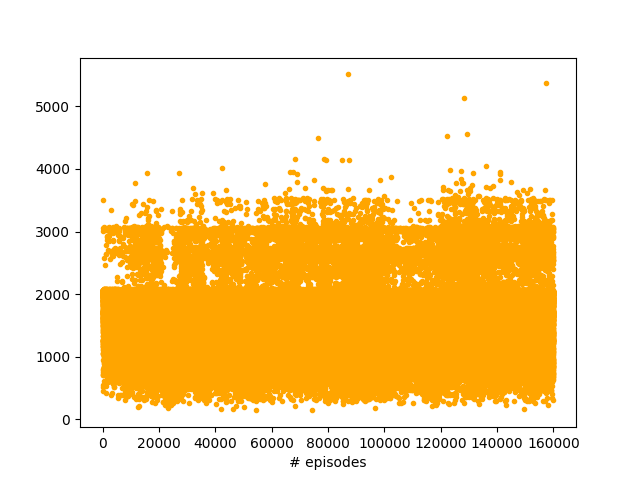
\includegraphics[scale=0.4]{05_experimental_results/05_images/ckpt-#0_big-net_replay_games_rewards.png}}
\caption{Game score}
\label{fig:0-2_reward}
\end{figure}

\begin{figure}[htbp]
\centerline{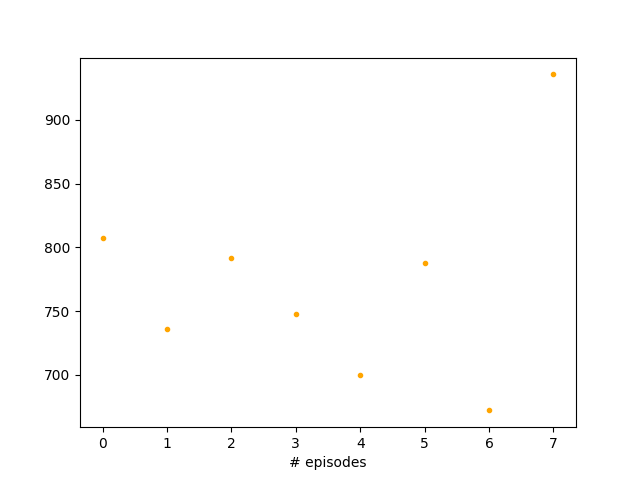
\includegraphics[scale=0.4]{05_experimental_results/05_images/ckpt-#0_big-net_replay_games_compute_percentiles_1000_rewards.png}}
\caption{Top 95 percentile game score, computed every 20000 episodes}
\label{fig:0-2_percentile}
\end{figure}

\begin{figure}[htbp]
\centerline{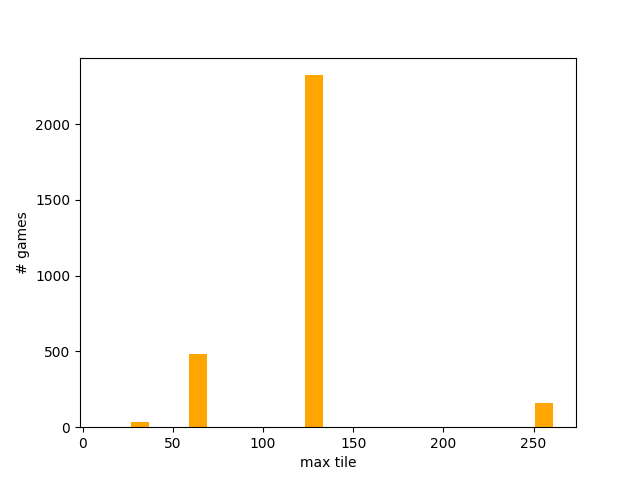
\includegraphics[scale=0.4]{05_experimental_results/05_images/ckpt-#0_big-net_replay_games_play_games_1000_ending_states.png}}
\caption{Number of game with specific max tile's value}
\label{fig:0-2_end_state}
\end{figure}

With this training the number of the 256 tiles is increased (see \ref{fig:0-2_end_state}) and the percentile value is increased (see \ref{fig:0-2_percentile}) too.

\subsection{Second implementation}
In the first implementation (see \ref{lab:second_net}) the \textit{policy network} is composed by eight hidden layers fully connected and the \textit{value network} composed by seven layers fully connected.

\subsubsection{First training}
$400000$ episodes:
\begin{figure}[htbp]
\centerline{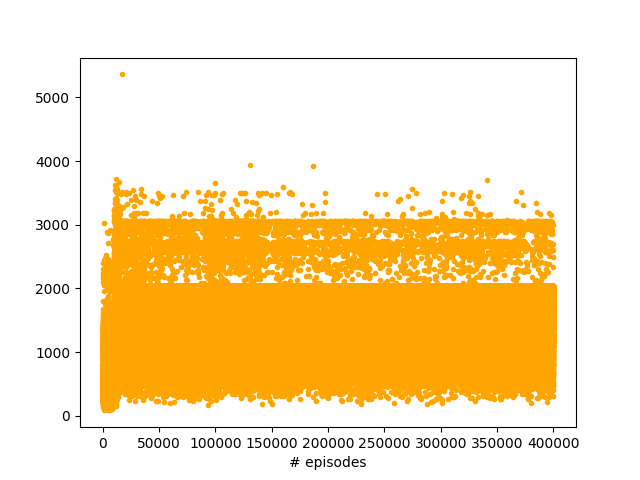
\includegraphics[scale=0.4]{05_experimental_results/05_images/ckpt-#1-0_norm_huge-net_rewards.png}}
\caption{Game score}
\label{fig:1-0_reward}
\end{figure}

\begin{figure}[htbp]
\centerline{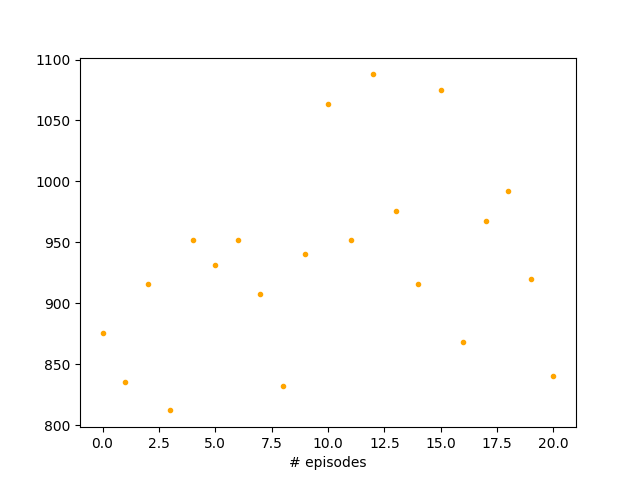
\includegraphics[scale=0.4]{05_experimental_results/05_images/ckpt-#1-0_norm_huge-net_compute_percentiles_1000_rewards.png}}
\caption{Top 95 percentile game score, computed every 20000 episodes}
\label{fig:1-0_percentile}
\end{figure}

\begin{figure}[htbp]
\centerline{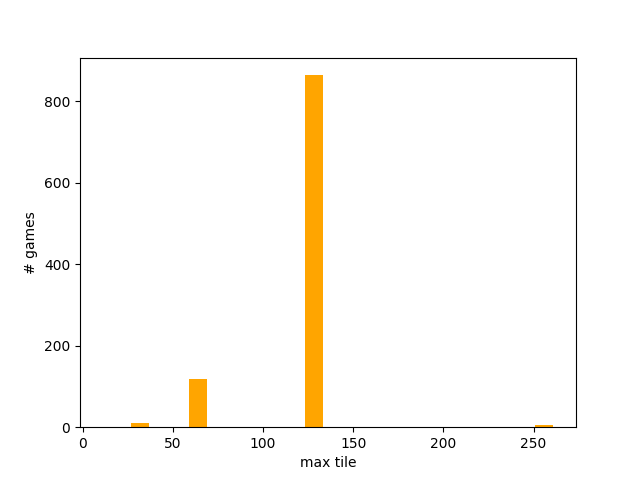
\includegraphics[scale=0.4]{05_experimental_results/05_images/ckpt-#1-0_norm_huge-net_play_games_1000_ending_states.png}}
\caption{Number of game with specific max tile's value}
\label{fig:1-0_end_state}
\end{figure}

The newly trained network exhibits better percentile values in the early episodes (fig \ref{fig:1-0_percentile}), but its performance growth rate is lower than that of the previous architecture (fig \ref{fig:0-1_percentile}).
When comparing the maximum tile plots, there are no discernible differences. However, the 128 tile is still the most prevalent (fig \ref{fig:1-0_end_state}).

\subsubsection{Second training}
$180000$ episodes using as starting board configuration $10000$ played games with probability $33\%$ (see \ref{lab:replay}):

\begin{figure}[htbp]
\centerline{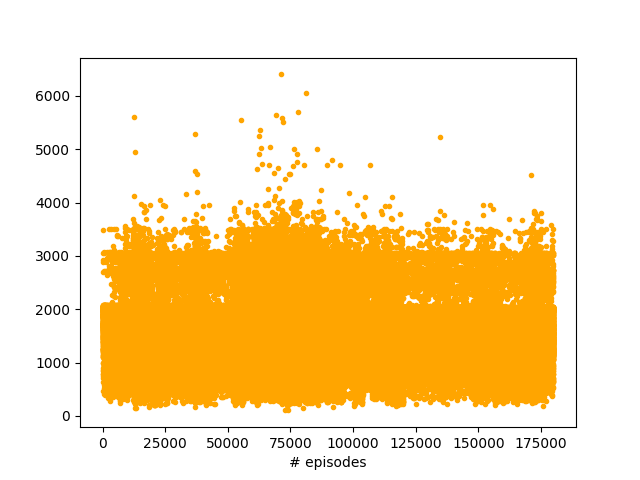
\includegraphics[scale=0.4]{05_experimental_results/05_images/ckpt-#1_big-net_replay_games_rewards.png}}
\caption{Game score}
\label{fig:1-1_reward}
\end{figure}

\begin{figure}[htbp]
\centerline{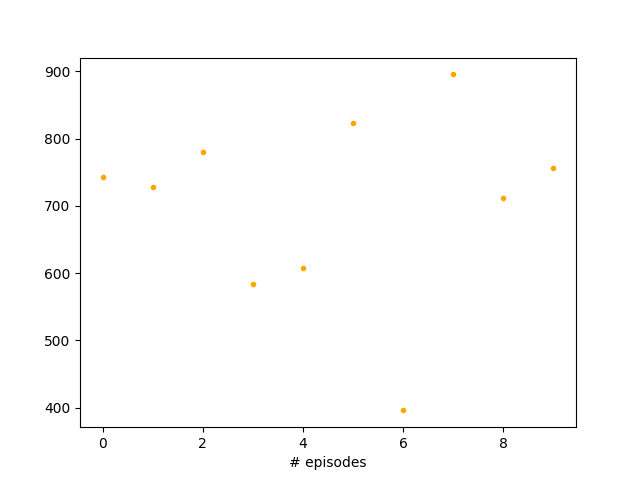
\includegraphics[scale=0.4]{05_experimental_results/05_images/ckpt-#1_big-net_replay_games_compute_percentiles_1000_rewards.png}}
\caption{Top 95 percentile game score, computed every 20000 episodes}
\label{fig:1-1_percentile}
\end{figure}

\begin{figure}[htbp]
\centerline{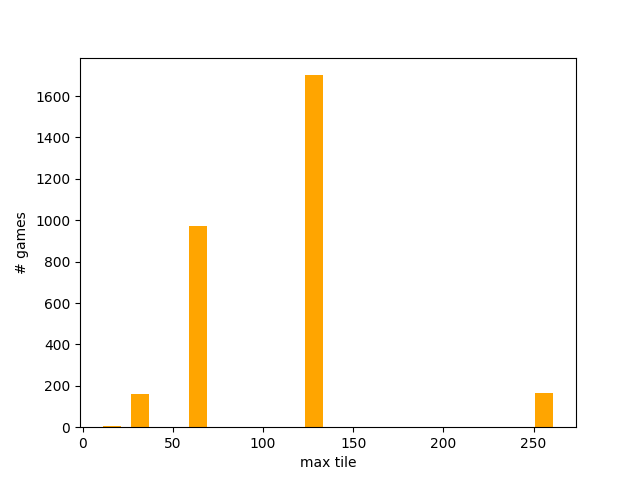
\includegraphics[scale=0.4]{05_experimental_results/05_images/ckpt-#1_big-net_replay_games_play_games_1000_ending_states.png}}
\caption{Number of game with specific max tile's value}
\label{fig:1-1_end_state}
\end{figure}

This training exhibits a substantial increase in the number of 256 tiles (fig \ref{fig:1-1_end_state}), while still maintaining the percentile values (fig \ref{fig:1-1_percentile}).

\section{Conclusion}
The stochastic nature of the 2048 game poses a challenge for the development of AI-based agents. This dissertation proposes two neural network architectures that employ distinct networks to address this challenge. Using played board configurations as initial state helps to improve the performances of the training. While the goal of reaching the tile 2048 was not achieved, the played board configurations have proven to be a valid help during the training.

\begin{thebibliography}{00}
\bibitem{ai-strat} Philip Rodgers, John Levine, An Investigation into 2048 AI Strategies
\bibitem{td-after} Marcin Szubert, Wojciech laskowski, Temporal Difference Learning of N-Tuple Networks for the Game 2048
\bibitem{td} Gerald Tesauro, Temporal DiWerence Learning and TD-Gammon
\bibitem{reinforce} Richard S. Sutton, David McAllester, Satinder Singh, Yishay Mansour, Policy Gradient Methods for Reinforcement Learning with Function Approximation
\bibitem{2048} Shilun Li, Veronica Peng, Playing 2048 With Reinforcement Learning
\end{thebibliography}

\end{document}
